\usepackage{amsfonts}

%----------------------------------------------------------------------------------------
%	PACKAGES AND OTHER DOCUMENT CONFIGURATIONS
%----------------------------------------------------------------------------------------


\documentclass[a4paper,12pt]{article}
\usepackage[english]{babel}
\usepackage[latin1]{inputenc}
\usepackage{amsmath}
\usepackage{amssymb}
\usepackage{amsfonts}
\usepackage{graphicx}
\usepackage[colorinlistoftodos]{todonotes}
\usepackage[toc,page]{appendix}
\usepackage{setspace}
\doublespacing
\usepackage{booktabs}
\usepackage{geometry}
\usepackage[bottom]{footmisc}
\usepackage{longtable}
\usepackage[demo]{graphicx}
\usepackage{subfig}
\usepackage{multirow}
\renewcommand{\arraystretch}{0.7}
\renewcommand{\labelitemi}{$\triangleright$}
 \geometry{
 a4paper,
 total={170mm,257mm},
 left=25mm,
 top=30mm,
 right=25mm,
 bottom=25mm,
 }
 \usepackage{hyperref}
 \hypersetup{
    bookmarks=true,         % show bookmarks bar?
    unicode=false,          % non-Latin characters in Acrobat’s bookmarks
    pdftoolbar=true,        % show Acrobat’s toolbar?
    pdfmenubar=true,        % show Acrobat’s menu?
    pdffitwindow=false,     % window fit to page when opened
    pdfstartview={FitH},    % fits the width of the page to the window
    pdftitle={Design_Report},    % title
    pdfauthor={Jacob Pichelman, Luca Poll},     % author
    pdfsubject={Subject},   % subject of the document
    pdfcreator={Creator},   % creator of the document
    pdfproducer={Producer}, % producer of the document
    pdfkeywords={keyword1, key2, key3}, % list of keywords
    pdfnewwindow=true,      % links in new PDF window
    colorlinks=false,       % false: boxed links; true: colored links
    linkcolor=red,          % color of internal links (change box color with linkbordercolor)
    citecolor=green,        % color of links to bibliography
    filecolor=magenta,      % color of file links
    urlcolor=cyan           % color of external links
}

	% biblatex
\usepackage[
       style=authoryear,
       natbib=true,
       maxcitenames=3,
       maxbibnames=11,
       backend=biber,
       pagetracker=page,
       hyperref=true,
       doi=true, 
       mergedate=compact, 
       firstinits=true
    ]{biblatex} 
	\usepackage{csquotes}
	\renewcommand*{\bibsetup}{
		\interlinepenalty=10000\relax % default is 5000
		\widowpenalty=10000\relax
		\clubpenalty=10000\relax
		\raggedbottom
		\frenchspacing
        \biburlsetup}
    \addbibresource{library.bib}

\begin{document}
\begin{titlepage}

\newcommand{\HRule}{\rule{\linewidth}{0.25mm}} % Defines a new command for the horizontal lines, change thickness here
\setlength{\topmargin}{-0.5in}
\center % Center everything on the page


\includegraphics[scale=0.75]{TSE.png}\\

%----------------------------------------------------------------------------------------
%	HEADING SECTIONS
%----------------------------------------------------------------------------------------
% \\[1.5cm]
\large \textsc{M2 EEE Panel Data}
\vspace{1.5cm}
% Name of your heading such as course name
\textsc{\large } % Minor heading such as course title

%----------------------------------------------------------------------------------------
%	TITLE SECTION
%----------------------------------------------------------------------------------------

\HRule \\[0.75cm]
{ \huge \bfseries Panel Data Replication Project}\\[0.5cm] % Title of your document
\HRule \\[1.75cm]

%----------------------------------------------------------------------------------------
%	AUTHOR SECTION
%----------------------------------------------------------------------------------------

\large\textsc{Andrew Boomer, \\ Jacob Pichelmann, \\Luca Poll} \\[1.5cm]

%----------------------------------------------------------------------------------------
%	DATE SECTION
%----------------------------------------------------------------------------------------

{\large \today}\\[0.5cm] % Date, change the \today to a set date if you want to be precise

\vfill % Fill the rest of the page with whitespace

\end{titlepage}

%-------------------------------------------------------------
% TABLE OF CONTENTS
\renewcommand{\contentsname}{Table of Contents}
\tableofcontents
\clearpage
%-----------------------------------------------------------------------------

\section{Introduction}
After the Arab spring and the related outbreak of unforeseen violence, conflict forecasting models were largely criticized, and it was argued that forecasting new civil wars might have reached a limit.
Mueller and Rauh (2018) though show in their paper "Reading between the lines: Prediction of political violence", that this might not be entirely true.
Their main argument is structured as follows: Conventional conflict forecasting models\footnote{\noindent They demonstrate their argument by replicating the following papers on conflict prediction: \begin{itemize}
    \item Miguel \& Satyanath (2011): Prediction through rainfall growth
    \item Besley \& Presson (2011): Prediction through proxies for external shocks and political constraints
    \item Goldstone et al. (2010): Prediction through political institution dummies, child mortality rates, share of population discriminated against and whether neighboring countries in conflict
    \item Ward et al. (2013): Event database on high-intensity and low-intensity conflict events used for analysis
    \item Chadefaux (2014): Conflict prediction through analysis of keyword count in newspaper text
\end{itemize}}, that rely on the overall variation in country fixed effect models, exhibit a bias towards predicting conflict onset to where conflict has occurred before. This is partially due to large country fixed effects and slow moving factors like population, ethnic fractionalization, climate, etc. that result in a large between variation. The forecasts are hence dominated by structural time-invariant (or slow moving) factors, neglecting valuable within variation. As a result these models are relatively good at predicting (biasedly) where conflict will happen, but not when it will happen. In order to improve the forecasting of the timing of conflict and generate an unbiased forecast, Mueller \& Rauh (2018) propose to isolate the within from the overall variation and use such to predict the onset of armed conflict and civil war. In order to obtain necessary within variation, they propose using topic modeling on newspaper text to create variables of the average distribution of topic shares observed in a country during a given year.



\section{Sample \& Data}
The key pillar of this analysis is the news data used to explain and predict conflict.
The authors use an unsupervised learning algorithm to distill topic shares out of a set of 700.000 newspaper articles from three internationally-reporting newspapers between 1975 and 2015: the Economist\footnote{174.450 articles from 1975 onward}, the New York Times\footnote{363.275 articles from 1980 onward} and the Washington Post\footnote{185.523 articles from 1977 onward}.
They start by processing the articles' contents with standard text mining techniques such as stemming words.\footnote{Stemming refers to the process of finding the common root of a word, i.e. “running”, “ran”, and “run” all become “run”.}
This leaves them with roughly 0.9 million tokens, which are then grouped into topics based on the latent Dirichlet allocation (LDA) method.
A topic then constitutes a probability distribution over words.
The result is intuitive, as one can imagine that an article covering "Sports" might indeed be more likely to contain words such as "score", "win" and "match" whereas an article concerned with "Conflict" could contain the phrases "war", "protest" and "military".
An indication of the resulting topic compositions is given by figure \ref{}.
The number of topics has to be specified beforehand, while the composition of topics is defined by the algorithm.
The authors choose to work with a final set of 15 topics.
Notably, each topic is a probability distribution over thousands of words, meaning the resulting topics have a certain level of depth that might increase their explanatory power, although being hard to intuitively assess.

The dependent variables on the other hand are constructed through battle-related deaths from the Uppsala Conflict Data Program (UCDP/PRIO).
Following their definition, armed conflict (dep. var. 1) is defined as a contested incompatibility that concerns government and/or territory over which the use of armed force between two parties, of which at least one is the government of a state, has resulted in at least 25 battle-related deaths in one calendar year.
Civil conflict (dep. var. 2) follows the same definition but requires at least 1.000 battle-related deaths in on calendar year. \\
% Talk about variation in data and place map here?

The panel summary statistics for these variables are given in Figure \ref{tab:xtsum}. (Provide futher explanation about the data)

\subsection{Data Preparation for Model} \label{data_prep}
The authors clean and prepare their data before estimation.
Some of these techniques we agree with, and others we have some theoretical issues with.
The pros and cons of their methods will be discussed in further detail after the initial replication section.

\begin{itemize}
    \item Observations with missing values in the topic shares are filled forward. If $\theta_{it}$ is missing, and $\theta_{it - 1}$ is not missing, then $\theta_{it} <- \theta_{it - 1}.$
    \item The chosen conflict variable itself is not used as the dependent variable. The authors specifically look at two scenarios, either the onset or the incidence of conflict.
        \begin{itemize}
            \item Onset of conflict is defined as $Conflict_{t} = 0$ and $Conflict_{t + 1} = 1$. After creating this onset variable, all observations where $Conflict_{t} = 1$ are removed.
            \item Incidence of Conflict is defined as $Conflict_{t} = 1$ and $Conflict_{t + 1} = 1$. After creating this incidence variable, missing conflict observations are removed.
            \item In our replication, we will narrow our focus to only the onset of conflict as the authors define it.
        \end{itemize}
    \item Observations where the average population over the entire sample is less than 1000, and where population data is missing are removed.
    \item Observations where there are zero words written, or where this data is missing, are removed.
    \item As a robustness check, the authors provide the option to restrict the sample to only countries who have experienced conflict at least once in the entire sample.
\end{itemize}

\section{Model}
The aim of the model is to create forecasts for an armed conflict/ civil war outbreak in period $T+1$ at period $T \in \{1995,..., 2013\}$.
To create this forecast, the full information set up to period $T$ is included into the forecast.
Therefore, the respective country-year topic shares $\theta_{n,i,T}$ are calculated for every newspaper sub-sample available up to period $T$\footnote{As the amount of available articles/ words expands in $T$, the basis for defining a topic through characteristic words in $T$ does also expand. Hence, the every topic characteristic and every topic distribution will vary at every $T$} for each country $i$ and topic $n$.
As a consequence, the following two steps are repeated at every $T$:

\noindent\textbf{Step 1: Estimate model and obtain fitted values}

\noindent From the model $y_{i,T+1} = \alpha + \beta_{i} + \theta_{i,T}\beta^{topics}$ the fitted values from the estimation based on the overall variation are obtained:

\begin{equation}
    \hat{y}_{i,T+1}^{overall} = \hat{\alpha} + \hat{\beta_i} + \theta_{i,T}\hat{\beta}^{topics}
\end{equation}

\noindent From these fitted values that rely on the overall variation, the fitted fixed effects are subtracted in order to obtain the fitted within model:

\begin{equation}
    \hat{y}_{i,T+1}^{within} = \hat{\alpha} + \theta_{i,T}\hat{\beta}^{topics}
\end{equation}

\noindent \textbf{Step 2: Produce forecast based on fitted values for period T+1}

\noindent 1) The fitted values are transformed into binary variables depending on cutoff value c\\
2) Compare forecast (binary variable) to realizations of armed conflict and civil war\\
3) Assess performance of overall and within model by considering forecasting performance for any given value c through ROC curves

\section{Replication Estimations}
In Table \ref{tab::armed} and Table \ref{tab::civil} we provide a replication of the models used by the authors.
They use a fixed effects model, and we show this compared to both a Pooled OLS model and a FE model where the topic shares are additionally interacted with an autocracy dummy. The interaction coefficients are omitted from the regression output.

We also replicated the ROC curve, comparing the false positive prediction rate to the true positive predictoin rate, in Figure \ref{rocfe}.
As the authors found in their research, the predictive quality of the estimation drops when excluding the between variation from the prediction.

\section{Enhancing the model}
We extend the authors' analysis by further exploiting their data to build a more holistic model.
We argue that the topic shares can serve as proxies for the true drivers of conflict: high dimensional, non-measurable events.
As seen in figure \ref{path} events affect both current and future conflicts as well as topics (i.e. reporting on said events).
We exploit these relationships to estimate a Blundell Bond model\footnote{We refrain from employing an Arellano Bond model since we expect the lagged value of conflict to have a strong impact on current conflict (i.e. the coefficient to be close to 1) in which case Arellano Bond does not perform well.} that can mitigate the most prominent trade-off when estimating conflict: the question of causality versus predictability.
By including the lagged value of conflict we can incorporate static factors that tend to perform well in explaining \textit{why} conflict takes place.
By regressing on lagged topic shares the model captures dynamic behavior stemming from events that \textit{cause} conflict.
The resulting model can be written as

\begin{equation}
    y_{it} = \alpha_i + \gamma y_{i, t-1} + \mathbf{\beta}\mathbf{\theta}_{i, t-1} + \varepsilon_{it}
\end{equation}

where all topic shares $\mathbf{\theta}$ are taken to be weakly exogenous.

\section{Accounting for country differences in reporting}
It is reasonable to assume that the effect of topic shares is heterogeneous across countries.
We make the assumption that the heterogeneity of the effect depends on the country's state of development.
This allows us to mitigate this issue by interacting topic shares with variables capturing each country's degree of development, such as child mortality and ...

\section{Limitations of this approach}
Naturally, this approach has its limitations that have to be kept in mind when evaluating the resulting estimates.
First of all, we employ a linear model to estimate a probability, which implies that the estimates are not bounded between 0 and 1.
A possible solution would be to estimate a random effects probit model and follow Wooldrigde (YEAR) in parametrizing the random effect.

Moreover, the Blundell Bond model assumes that the initial value of conflict is drawn from a steady state distribution.
This is unlikely to hold in the given context.


\newpage

\begin{appendix}
    \section{Figures and Tables}
    \begin{longtable}{lllrrrr}

\toprule
               &        &  Mean &  Std. Dev. &    Min &   Max &  Observations \\
\textbf{Variable} & \textbf{Type} &       &            &        &       &               \\
\midrule
\multirow{3}{*}{\textbf{Armed Conflict}} & \textbf{overall} & 0.142 &      0.349 &  0.000 & 1.000 &          7520 \\
               & \textbf{between} &       &      0.020 &  0.106 & 0.186 &            40 \\
               & \textbf{within} &       &      0.349 & -0.044 & 1.036 &           188 \\
\cline{1-7}
\multirow{3}{*}{\textbf{Civil War}} & \textbf{overall} & 0.060 &      0.237 &  0.000 & 1.000 &          7520 \\
               & \textbf{between} &       &      0.024 &  0.027 & 0.112 &            40 \\
               & \textbf{within} &       &      0.236 & -0.052 & 1.033 &           188 \\
\cline{1-7}
\multirow{3}{*}{\textbf{Topic 1 Share}} & \textbf{overall} & 0.053 &      0.039 &  0.007 & 0.560 &          6639 \\
               & \textbf{between} &       &      0.005 &  0.046 & 0.063 &            39 \\
               & \textbf{within} &       &      0.038 & -0.002 & 0.561 &           185 \\
\cline{1-7}
\multirow{3}{*}{\textbf{Topic 2 Share}} & \textbf{overall} & 0.073 &      0.041 &  0.010 & 0.559 &          6639 \\
               & \textbf{between} &       &      0.010 &  0.050 & 0.089 &            39 \\
               & \textbf{within} &       &      0.040 &  0.004 & 0.549 &           185 \\
\cline{1-7}
\multirow{3}{*}{\textbf{Topic 3 Share}} & \textbf{overall} & 0.043 &      0.049 &  0.006 & 0.454 &          6639 \\
               & \textbf{between} &       &      0.003 &  0.038 & 0.051 &            39 \\
               & \textbf{within} &       &      0.049 &  0.004 & 0.451 &           185 \\
\cline{1-7}
\multirow{3}{*}{\textbf{Topic 4 Share}} & \textbf{overall} & 0.060 &      0.068 &  0.009 & 0.663 &          6639 \\
               & \textbf{between} &       &      0.012 &  0.032 & 0.080 &            39 \\
               & \textbf{within} &       &      0.067 & -0.006 & 0.663 &           185 \\
\cline{1-7}
\multirow{3}{*}{\textbf{Topic 5 Share}} & \textbf{overall} & 0.069 &      0.045 &  0.004 & 0.468 &          6639 \\
               & \textbf{between} &       &      0.008 &  0.045 & 0.081 &            39 \\
               & \textbf{within} &       &      0.045 & -0.003 & 0.476 &           185 \\
\cline{1-7}
\multirow{3}{*}{\textbf{Topic 6 Share}} & \textbf{overall} & 0.063 &      0.052 &  0.009 & 0.765 &          6639 \\
               & \textbf{between} &       &      0.011 &  0.036 & 0.081 &            39 \\
               & \textbf{within} &       &      0.051 & -0.003 & 0.774 &           185 \\
\cline{1-7}
\multirow{3}{*}{\textbf{Topic 7 Share}} & \textbf{overall} & 0.074 &      0.047 &  0.007 & 0.514 &          6639 \\
               & \textbf{between} &       &      0.006 &  0.063 & 0.086 &            39 \\
               & \textbf{within} &       &      0.046 & -0.005 & 0.509 &           185 \\
\cline{1-7}
\multirow{3}{*}{\textbf{Topic 8 Share}} & \textbf{overall} & 0.070 &      0.052 &  0.007 & 0.426 &          6639 \\
               & \textbf{between} &       &      0.006 &  0.058 & 0.084 &            39 \\
               & \textbf{within} &       &      0.051 & -0.006 & 0.420 &           185 \\
\cline{1-7}
\multirow{3}{*}{\textbf{Topic 9 Share}} & \textbf{overall} & 0.074 &      0.054 &  0.010 & 0.514 &          6639 \\
               & \textbf{between} &       &      0.012 &  0.058 & 0.116 &            39 \\
               & \textbf{within} &       &      0.053 & -0.024 & 0.519 &           185 \\
\cline{1-7}
\multirow{3}{*}{\textbf{Topic 10 Share}} & \textbf{overall} & 0.065 &      0.051 &  0.007 & 0.612 &          6639 \\
               & \textbf{between} &       &      0.008 &  0.053 & 0.092 &            39 \\
               & \textbf{within} &       &      0.051 & -0.009 & 0.605 &           185 \\
\cline{1-7}
\multirow{3}{*}{\textbf{Topic 11 Share}} & \textbf{overall} & 0.063 &      0.046 &  0.005 & 0.407 &          6639 \\
               & \textbf{between} &       &      0.010 &  0.047 & 0.082 &            39 \\
               & \textbf{within} &       &      0.044 & -0.008 & 0.410 &           185 \\
\cline{1-7}
\multirow{3}{*}{\textbf{Topic 12 Share}} & \textbf{overall} & 0.075 &      0.069 &  0.004 & 0.653 &          6639 \\
               & \textbf{between} &       &      0.017 &  0.058 & 0.135 &            39 \\
               & \textbf{within} &       &      0.067 & -0.044 & 0.654 &           185 \\
\cline{1-7}
\multirow{3}{*}{\textbf{Topic 13 Share}} & \textbf{overall} & 0.089 &      0.090 &  0.008 & 0.623 &          6639 \\
               & \textbf{between} &       &      0.010 &  0.070 & 0.103 &            39 \\
               & \textbf{within} &       &      0.090 & -0.001 & 0.614 &           185 \\
\cline{1-7}
\multirow{3}{*}{\textbf{Topic 14 Share}} & \textbf{overall} & 0.067 &      0.048 &  0.007 & 0.582 &          6639 \\
               & \textbf{between} &       &      0.005 &  0.058 & 0.076 &            39 \\
               & \textbf{within} &       &      0.048 &  0.006 & 0.579 &           185 \\
\cline{1-7}
\multirow{3}{*}{\textbf{Topic 15 Share}} & \textbf{overall} & 0.061 &      0.055 &  0.006 & 0.437 &          6639 \\
               & \textbf{between} &       &      0.007 &  0.048 & 0.075 &            39 \\
               & \textbf{within} &       &      0.055 & -0.006 & 0.429 &           185 \\
\bottomrule
\caption{Panel Data Summary}
\label{tab:xtsum}
\end{longtable}

    \clearpage
    \newpage

    \begin{figure}[!h]
        \caption{Path Diagram of Model Hypothesis}
        \centering
        \tikzstyle{box} = [rectangle, rounded corners, minimum width=1cm, minimum height=1cm,text centered, draw=black]
\tikzstyle{arrow} = [thick,->,>=stealth]

\begin{tikzpicture}[node distance = 2cm]
    \node (Yt) [box, fill = yellow!80!black, text width = 2cm] {\small $Conflict_{t}$};
    \node (Yt+1) [box, right of = Yt, node distance = 3.5cm, fill = yellow!80!black, text width = 2cm] {\small $Conflict_{t + 1}$};
    \node (Yt+2) [box, right of = Yt+1, node distance = 3.5cm, fill = yellow!80!black, text width = 2cm] {\small $Conflict_{t + 2}$};
    \node (YT) [box, right of = Yt+2, node distance = 3.5cm, fill = yellow!80!black, text width = 2cm] {\small $Conflict_{T}$};

    \node (Et) [box, below of = Yt, node distance = 4cm, fill = yellow!80!black, text width = 2cm] {\small $Events_{t}$};
    \node (Et+1) [box, right of = Et, node distance = 3.5cm, fill = yellow!80!black, text width = 2cm] {\small $Events_{t + 1}$};
    \node (Et+2) [box, right of = Et+1, node distance = 3.5cm, fill = yellow!80!black, text width = 2cm] {\small $Events_{t + 2}$};
    \node (ET) [box, right of = Et+2, node distance = 3.5cm, fill = yellow!80!black, text width = 2cm] {\small $Events_{T}$};

    \node (Xt) [box, below of = Et, node distance = 2.5cm, fill = yellow!80!black, text width = 2cm] {\small $\textbf{Theta}_{t}$};
    \node (Xt+1) [box, right of = Xt, node distance = 3.5cm, fill = yellow!80!black, text width = 2cm] {\small $\textbf{Theta}_{t + 1}$};
    \node (Xt+2) [box, right of = Xt+1, node distance = 3.5cm, fill = yellow!80!black, text width = 2cm] {\small $\textbf{Theta}_{t + 2}$};
    \node (XT) [box, right of = Xt+2, node distance = 3.5cm, fill = yellow!80!black, text width = 2cm] {\small $\textbf{Theta}_{T}$};
    
    \node (X) [fit = (Xt) (XT), draw, black, dotted] {};
    \node (Y) [fit = (Yt) (YT), draw, black, dotted] {};
    \node (E) [fit = (Et) (ET), draw, black, dotted] {};

    \node (alpha) [box, below left = 1cm and 0.5cm of Yt, fill = yellow!80!black, text width = 0.75cm] {\small $\alpha_{i}$};
    \node (epsilon) [box, right of = YT, node distance = 3cm, fill = yellow!80!black, text width = 0.75cm] {\small $\epsilon_{it}$};

    \draw [arrow] (Yt) -- (Yt+1);
    \draw [arrow] (Yt+1) -- (Yt+2);
    \draw [arrow] (Yt+2) -- (YT);

    \draw [arrow] (Et) -- (Yt+1);
    \draw [arrow] (Et+1) -- (Yt+2);
    \draw [arrow] (Et+2) -- (YT);

    \draw [arrow] (Yt) -- (Et+1);
    \draw [arrow] (Yt+1) -- (Et+2);
    \draw [arrow] (Yt+2) -- (ET);

    \draw [arrow] (Et) -- (Et+1);
    \draw [arrow] (Et+1) -- (Et+2);
    \draw [arrow] (Et+2) -- (ET);

    \draw [arrow, <->, blue] (Et) -- (Yt);
    \draw [arrow, <->, blue] (Et+1) -- (Yt+1);
    \draw [arrow, <->, blue] (Et+2) -- (Yt+2);
    \draw [arrow, <->, blue] (ET) -- (YT);

    \draw [arrow, <-, green!45!black] (Xt) -- (Et);
    \draw [arrow, <-, green!45!black] (Xt+1) -- (Et+1);
    \draw [arrow, <-, green!45!black] (Xt+2) -- (Et+2);
    \draw [arrow, <-, green!45!black] (XT) -- (ET);

    \draw [arrow, <-, green!45!black, dotted] (Xt+1) -- (Et);
    \draw [arrow, <-, green!45!black, dotted] (Xt+2) -- (Et+1);
    \draw [arrow, <-, green!45!black, dotted] (XT) -- (Et+2);

    \draw[<->, bend left, thick] (alpha.north) to (Y.west);
    \draw[<->, bend right, thick] (alpha.south) to (E.west);

    \draw[<->, thick] (epsilon.west) to (Y.east);

    % \draw[arrow] (IV) -- (log_items) node[midway, fill = white, inner sep = 0pt] {IV};
    % \draw[arrow, <->] (unobs) -- (log_items);
\end{tikzpicture}
        \label{path}
    \end{figure}

    \clearpage
    \newpage

    \begin{table}[!h]
        \caption{Initial Panel Models: Armed Conflict}
        \centering
        \begin{center}
\begin{tabular}{lccc}
\\[-1.8ex]\hline
& $\textbf{Pooled}$& $\textbf{FE}$& $\textbf{FEInteract}$\\
 \hline \hline 
& \multicolumn{3}{c}{Armed Conflict} \\
\hline \\[-1.8ex]
Constant & -0.2615$^{***}$ & -0.2195$^{***}$ & -0.2193$^{***}$ \\
 & (0.0609)& (0.0742)& (0.0795)\\ 
\\Topic 2 Share & 0.2588$^{***}$ & 0.2625$^{**}$ & 0.2920$^{***}$ \\
 & (0.0767)& (0.1038)& (0.1107)\\ 
\\Topic 3 Share & 0.1760$^{**}$ & 0.2651$^{*}$ & 0.2395 \\
 & (0.0857)& (0.1419)& (0.1542)\\ 
\\Topic 4 Share & 0.5330$^{***}$ & 0.3668$^{***}$ & 0.4174$^{***}$ \\
 & (0.1304)& (0.1193)& (0.1224)\\ 
\\Topic 5 Share & 0.1846$^{***}$ & 0.2132$^{**}$ & 0.1819$^{*}$ \\
 & (0.0686)& (0.0841)& (0.1003)\\ 
\\Topic 6 Share & 0.3911$^{**}$ & 0.1447 & 0.2605$^{*}$ \\
 & (0.1710)& (0.1233)& (0.1413)\\ 
\\Topic 7 Share & 0.1748$^{**}$ & 0.2595$^{*}$ & 0.2531$^{*}$ \\
 & (0.0680)& (0.1362)& (0.1459)\\ 
\\Topic 8 Share & 0.3066$^{***}$ & 0.2768$^{***}$ & 0.2715$^{***}$ \\
 & (0.0763)& (0.0883)& (0.0894)\\ 
\\Topic 9 Share & 0.1820$^{***}$ & 0.1710$^{*}$ & 0.1878$^{**}$ \\
 & (0.0641)& (0.0883)& (0.0891)\\ 
\\Topic 10 Share & 0.2764$^{***}$ & 0.2381$^{**}$ & 0.2535$^{**}$ \\
 & (0.0955)& (0.1146)& (0.1238)\\ 
\\Topic 11 Share & 1.0280$^{***}$ & 0.8449$^{***}$ & 0.8301$^{***}$ \\
 & (0.1670)& (0.1935)& (0.2011)\\ 
\\Topic 12 Share & 0.2100$^{***}$ & 0.2001$^{**}$ & 0.1826$^{*}$ \\
 & (0.0793)& (0.0925)& (0.1011)\\ 
\\Topic 13 Share & 0.2398$^{**}$ & 0.2287$^{**}$ & 0.2037$^{**}$ \\
 & (0.0966)& (0.0950)& (0.0985)\\ 
\\Topic 14 Share & 0.3517$^{***}$ & 0.2141$^{**}$ & 0.1217 \\
 & (0.0991)& (0.1018)& (0.1186)\\ 
\\Topic 15 Share & 0.2953$^{***}$ & 0.2827$^{***}$ & 0.2915$^{**}$ \\
 & (0.0803)& (0.1091)& (0.1263)\\ 
\hline \\[-1.8ex]
 \\ Included Effects:  & Time & Entity, Time & Entity, Time\\ R-Squared:  & 0.042&0.015&0.023\\ Observations:  & 4486&4486&4348\end{tabular}
\end{center}Cluster Robust Standard Errors
        \label{tab::armed}
    \end{table}

    \begin{table}[!h]
        \caption{Initial Panel Models: Civil War}
        \centering
        \begin{center}
\begin{tabular}{lccc}
\\[-1.8ex]\hline
& $\textbf{Pooled}$& $\textbf{FE}$& $\textbf{FEInteract}$\\
 \hline \hline 
& \multicolumn{3}{c}{Civil War} \\
\hline \\[-1.8ex]
Constant & -0.0674 & -0.1259$^{**}$ & -0.1293$^{**}$ \\
 & (0.0844)& (0.0596)& (0.0622)\\ 
\\Topic 2 Share & 0.0641 & 0.1564$^{*}$ & 0.1643$^{**}$ \\
 & (0.0860)& (0.0804)& (0.0831)\\ 
\\Topic 3 Share & 0.0750 & 0.2212$^{**}$ & 0.2147$^{**}$ \\
 & (0.1008)& (0.0913)& (0.0948)\\ 
\\Topic 4 Share & 0.2844$^{**}$ & 0.2748$^{***}$ & 0.3124$^{***}$ \\
 & (0.1109)& (0.0876)& (0.0995)\\ 
\\Topic 5 Share & 0.0580 & 0.1866$^{***}$ & 0.2019$^{**}$ \\
 & (0.0875)& (0.0666)& (0.0787)\\ 
\\Topic 6 Share & 0.0698 & 0.0017 & 0.0650 \\
 & (0.1343)& (0.1277)& (0.1146)\\ 
\\Topic 7 Share & 0.0074 & -0.0088 & -0.0226 \\
 & (0.0891)& (0.0913)& (0.0899)\\ 
\\Topic 8 Share & 0.0001 & 0.0671 & 0.0508 \\
 & (0.1003)& (0.0702)& (0.0694)\\ 
\\Topic 9 Share & 0.0534 & 0.1182$^{*}$ & 0.1336$^{**}$ \\
 & (0.0898)& (0.0629)& (0.0659)\\ 
\\Topic 10 Share & 0.0218 & 0.0919 & 0.0988 \\
 & (0.0990)& (0.0841)& (0.0870)\\ 
\\Topic 11 Share & 0.4905$^{***}$ & 0.5722$^{***}$ & 0.5778$^{***}$ \\
 & (0.1579)& (0.1574)& (0.1611)\\ 
\\Topic 12 Share & 0.0533 & 0.1118 & 0.1106 \\
 & (0.0952)& (0.0742)& (0.0772)\\ 
\\Topic 13 Share & 0.0352 & 0.1570$^{**}$ & 0.1615$^{**}$ \\
 & (0.0900)& (0.0730)& (0.0728)\\ 
\\Topic 14 Share & 0.0712 & 0.0972 & 0.0856 \\
 & (0.1183)& (0.0762)& (0.0843)\\ 
\\Topic 15 Share & 0.0732 & 0.1601$^{**}$ & 0.1157 \\
 & (0.0814)& (0.0661)& (0.0745)\\ 
\hline \\[-1.8ex]
 \\ Included Effects:  & Time & Entity, Time & Entity, Time\\ R-Squared:  & 0.036&0.020&0.027\\ Observations:  & 5062&5062&4924\end{tabular}
\end{center}Cluster Robust Standard Errors
        \label{tab::civil}
    \end{table}

    \begin{figure}[!h]
        \centering
        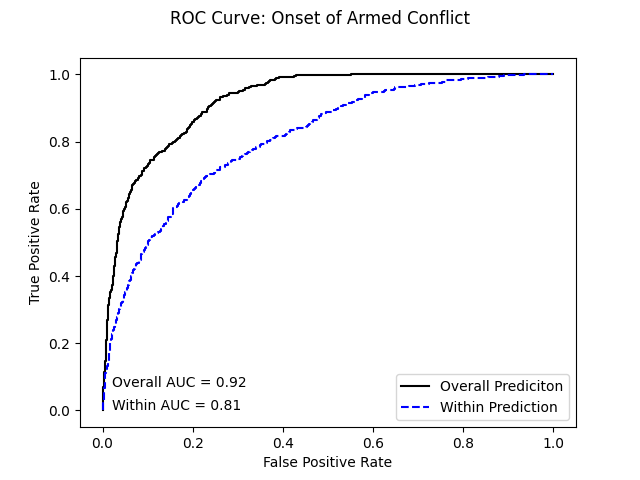
\includegraphics{ROC_FE.png}
        \caption{ROC Curve}
        \label{rocfe}
    \end{figure}

    \begin{table}[!h]
        \caption{Blundell-Bond System Models}
        \begin{minipage}{.5\linewidth}
          \begin{center}
\begin{tabular}{lc}
\\[-1.8ex]\hline
& $\textbf{GMM}$\\
 \hline \hline 
& \multicolumn{1}{c}{Armed Conflict} \\
\hline \\[-1.8ex]
Lag of Topic 2 Share & 0.0546 \\
 & (0.0405)\\ 
\\Lag of Topic 3 Share & 0.1603 \\
 & (0.0981)\\ 
\\Lag of Topic 4 Share & -0.0218 \\
 & (0.0838)\\ 
\\Lag of Topic 5 Share & 0.1205$^{**}$ \\
 & (0.0555)\\ 
\\Lag of Topic 6 Share & 0.3156$^{***}$ \\
 & (0.0971)\\ 
\\Lag of Topic 7 Share & 0.2127$^{**}$ \\
 & (0.1084)\\ 
\\Lag of Topic 8 Share & -0.0522 \\
 & (0.0465)\\ 
\\Lag of Topic 9 Share & -0.1058$^{***}$ \\
 & (0.0378)\\ 
\\Lag of Topic 10 Share & 0.0705 \\
 & (0.0528)\\ 
\\Lag of Topic 11 Share & 0.3721$^{***}$ \\
 & (0.1006)\\ 
\\Lag of Topic 12 Share & 0.0105 \\
 & (0.0559)\\ 
\\Lag of Topic 13 Share & 0.0540 \\
 & (0.0746)\\ 
\\Lag of Topic 14 Share & -0.0588 \\
 & (0.0566)\\ 
\\Lag of Topic 15 Share & 0.0306 \\
 & (0.0444)\\ 
\\Lag of Armed Conflict & 0.5891$^{***}$ \\
 & (0.0234)\\ 
\hline \\[-1.8ex]
 \\ Included Effects:  & Time, Entity\\ R-Squared:  & 0.403\\ Observations:  & 8954\end{tabular}
\end{center}Cluster Robust Standard Errors
        \end{minipage}%
        \begin{minipage}{.5\linewidth}
            \begin{center}
\begin{tabular}{lc}
\\[-1.8ex]\hline
& $\textbf{GMM}$\\
 \hline \hline 
& \multicolumn{1}{c}{Civil War} \\
\hline \\[-1.8ex]
Lag of Topic 2 Share & 0.0418 \\
 & (0.0268)\\ 
\\Lag of Topic 3 Share & -0.1096$^{***}$ \\
 & (0.0395)\\ 
\\Lag of Topic 4 Share & 0.0353 \\
 & (0.0362)\\ 
\\Lag of Topic 5 Share & 0.0079 \\
 & (0.0250)\\ 
\\Lag of Topic 6 Share & 0.0237 \\
 & (0.0509)\\ 
\\Lag of Topic 7 Share & -0.0342 \\
 & (0.0269)\\ 
\\Lag of Topic 8 Share & -0.0232 \\
 & (0.0278)\\ 
\\Lag of Topic 9 Share & -0.0312 \\
 & (0.0226)\\ 
\\Lag of Topic 10 Share & -0.0432 \\
 & (0.0265)\\ 
\\Lag of Topic 11 Share & 0.3930$^{***}$ \\
 & (0.0668)\\ 
\\Lag of Topic 12 Share & -0.0430 \\
 & (0.0307)\\ 
\\Lag of Topic 13 Share & -0.0522$^{*}$ \\
 & (0.0298)\\ 
\\Lag of Topic 14 Share & -0.0334 \\
 & (0.0360)\\ 
\\Lag of Topic 15 Share & 0.0142 \\
 & (0.0310)\\ 
\\Lag of Civil War & 0.6720$^{***}$ \\
 & (0.0141)\\ 
\hline \\[-1.8ex]
 \\ Included Effects:  & Time, Entity\\ R-Squared:  & 0.197\\ Observations:  & 8954\end{tabular}
\end{center}Cluster Robust Standard Errors
        \end{minipage}
        \label{gmm_mods}
    \end{table}

    \clearpage
    \newpage

    \begin{figure}[!h]
        \centering
        \includegraphics{thetas_total.png}
        \caption{Topic Shares over Time}
        \label{tstopics}
    \end{figure}

\end{appendix}

\clearpage

\newpage

\section*{References}[!h]
Besley, Timothy and Torsten Persson. 2011. Pillars of prosperity: The political economics \newline \indent of development clusters. Princeton University Press.\vspace{0.25cm}

\noindent Chadefaux, Thomas. 2014. "Early warning signals for war in the news." Journal of Peace \newline \indent Research 51(1):5-18.\vspace{0.25cm}

\noindent Goldstone, Jack A, Robert H Bates, David L Epstein, Ted Robert Gurr, Michael B Lustik, \newline \indent Monty G Marshall, Jay Ulfelder and Mark Woodward. 2010. "A global model for \newline \indent forecasting political instability." American Journal of Political Science 54(1):190-208.\vspace{0.25cm}

\noindent Miguel, Edward and Shanker Satyanath. 2011. "Re-examining economic shocks and civil \newline \indent conflict." American Economic Journal: Applied Economics 3(4):228-232.\vspace{0.25cm}

\noindent Mueller, H., \& Rauh, C. (2018). "Reading Between the Lines: Prediction of Political \newline \indent Violence Using Newspaper Text." American Political Science Review, 112(2), 358-375. \newline \indent doi:10.1017/S0003055417000570\vspace{0.25cm}

\noindent Ward, Michael D, Nils W Metternich, Cassy L Dorff, Max Gallop, Florian M Hollenbach, \newline \indent Anna Schultz and Simon Weschle. 2013. "Learning from the past and stepping into \newline \indent the future: Toward a new generation of conflict prediction." International Studies \newline \indent Review 15(4):473-490.

\clearpage

\end{document}